\section{Algorithm}

\begin{frame}[t]{Getting started}
    \framesubtitle{What do we need?}
	
    \begin{itemize}
   	\item<+->{
   		\stress{Select parameter space \& observable}:\\
   		$\lra$ Generate histograms for each point in parameter space
   	}

    \item<+->{
    	\bigskip
        \stress{Quantify \enquote{similar} histograms} {\color{purple}(\emph{metric})}:\\
    	$\lra$ Similarity test\\
        $\phantom{\lra}$ {\small e.g. $\chi^2$ test, Kolmogorov test, \dots}
	}
    
    \item<+->{
    	\bigskip
    	\stress{Build up groups} {\color{purple}(\emph{clusters})} of similar distributions:\\
    	$\lra$ Clustering algorithm\\
        $\phantom{\lra}$ {\small e.g. Hierarchical clustering, \dots}
    }
    
    \item<+->{
        \bigskip
        \stress{Select representatives} {\color{purple}(\emph{benchmark points})} from each cluster
    }
    
    \item<+->{
    	\bigskip
    	\stress{How many} clusters do we want?\\
    	$\lra$ Add experimental error expectation\\
    	$\lra$ Keep as many clusters as we can distinguish
    }
    \end{itemize}
\end{frame}

\begin{frame}{The metric}{Similarity between distributions}
	\begin{itemize}
		\item Let's take two points in parameter space $p_{1,2}$ and their corresponding kinematic histograms \hhl{$H_{1,2}$} with bin contents \hhl{$n_{1i}$}
		\item How well would we be able to distinguish between both cases?
		\item Estimate experimental uncertainties when conducting measurement \srem{(under the assumption that $H_k$ is the truth distribution)} $\lra$ Covariance matrices \hhl{$\Sigma_{1,2}$} 
		\item Let's assume that the measurement would indeed return the expectation value $H_{1,2}$ with $\Sigma_{1,2}$
		\item Use a test statistic that allows to include uncertainties.  
		\item In the paper we only compared the shape of the histograms $\lra$ test statistic shouldn't depend on normalization
		\item Used a \hhl{$\chi^2$ test with normalization} \srem{(and made some mistakes in the paper)}	
	\end{itemize}
\end{frame}

\begin{frame}{The metric}{$\chi^2$ metric}
	\begin{itemize}
		\item Normal $\chi^2$ distance: 
		\begin{align}
		\chi^2(H_1, H_2) = \chi^2(H_1, H_2) = \sum_{i=1}^N \frac{(n_{2i}-n_{1i})^2}{\sigma_{2i}^2+\sigma_{2i}^2}
		\label{eq:chi2_nonorm}
		\end{align}
		$\chi^2(H_1,H_2)\hhl{\sim \chi^2_N}$ under null hypothesis $E[n_{2i}]=E[n_{1i}]$
		\item \hhl{Normalized} ($\Sigma_k = \operatorname{diag}\sigma_{ki}^2$):
		\begin{align}
		  \chi^2(H_1, H_2) = \sum_{i=1}^N \frac{(N_1n_{2i}-N_2n_{1i})^2}{N_1^2\sigma_{2i}^2+N_2^2\sigma_{2i}^2}\,.
		  \label{eq:chi2_root}
		\end{align}
		\srem{(same as using \eqref{eq:chi2_nonorm} on normalized histograms $n_{ki}/N_k$)}
		\item This approximates (!) a $\chi^2_{N-1}$ distribution under null hypothesis \srem{(note reduced degrees of freedom -- wrong in the paper)}
		\item What about \hhl{correlations} induced by the measurement? $\lra$ In the paper we argue about \enquote{unrotating} them to use \eqref{eq:chi2_root}. Unfortunately this is \emph{nonsense} \srem{(and my fault -- luckily it doesn't affect the examples)}. 
	\end{itemize}
\end{frame}

\begin{frame}{The metric}
	\begin{itemize}
		\item Let's handle correlations properly: 
		\begin{itemize}
			\item Define $\Delta_i=\displaystyle\frac{n_{1i}}{N_1}-\frac{n_{2i}}{N_2}$
			\item Then $\operatorname{Cov}(\Delta_i, \Delta_j)=\displaystyle \frac{\Sigma_1}{N_1^2} + \frac{\Sigma_2}{N_2^2}$
			\item Now $\chi^2(H_1,H_2):= \hhl{\sum_{i,j=1}^N \Delta_i (\Sigma^{-1})_{ij} \Delta_j}$ is approximately $\chi^2_{N-1}$ distributed
		\end{itemize}
		\item Fixed in \texttt{ClusterKinG} v1.1.0
		%\item This time we properly validated our implementation
	\end{itemize}
\end{frame}

\begin{frame}{The metric}{Slight tangent: Normalized $\chi^2$ metric can be dangerous}
	\begin{itemize}
		\item It should be noted that the \emph{approximation} $\sim \chi^2_{N-1}$ can break down if uncertainties are very unbalanced
	\end{itemize}
	%\vspace{-0.1cm}
	\begin{changemargin}{-1cm}{-1cm}
		\centering
	\only<1>{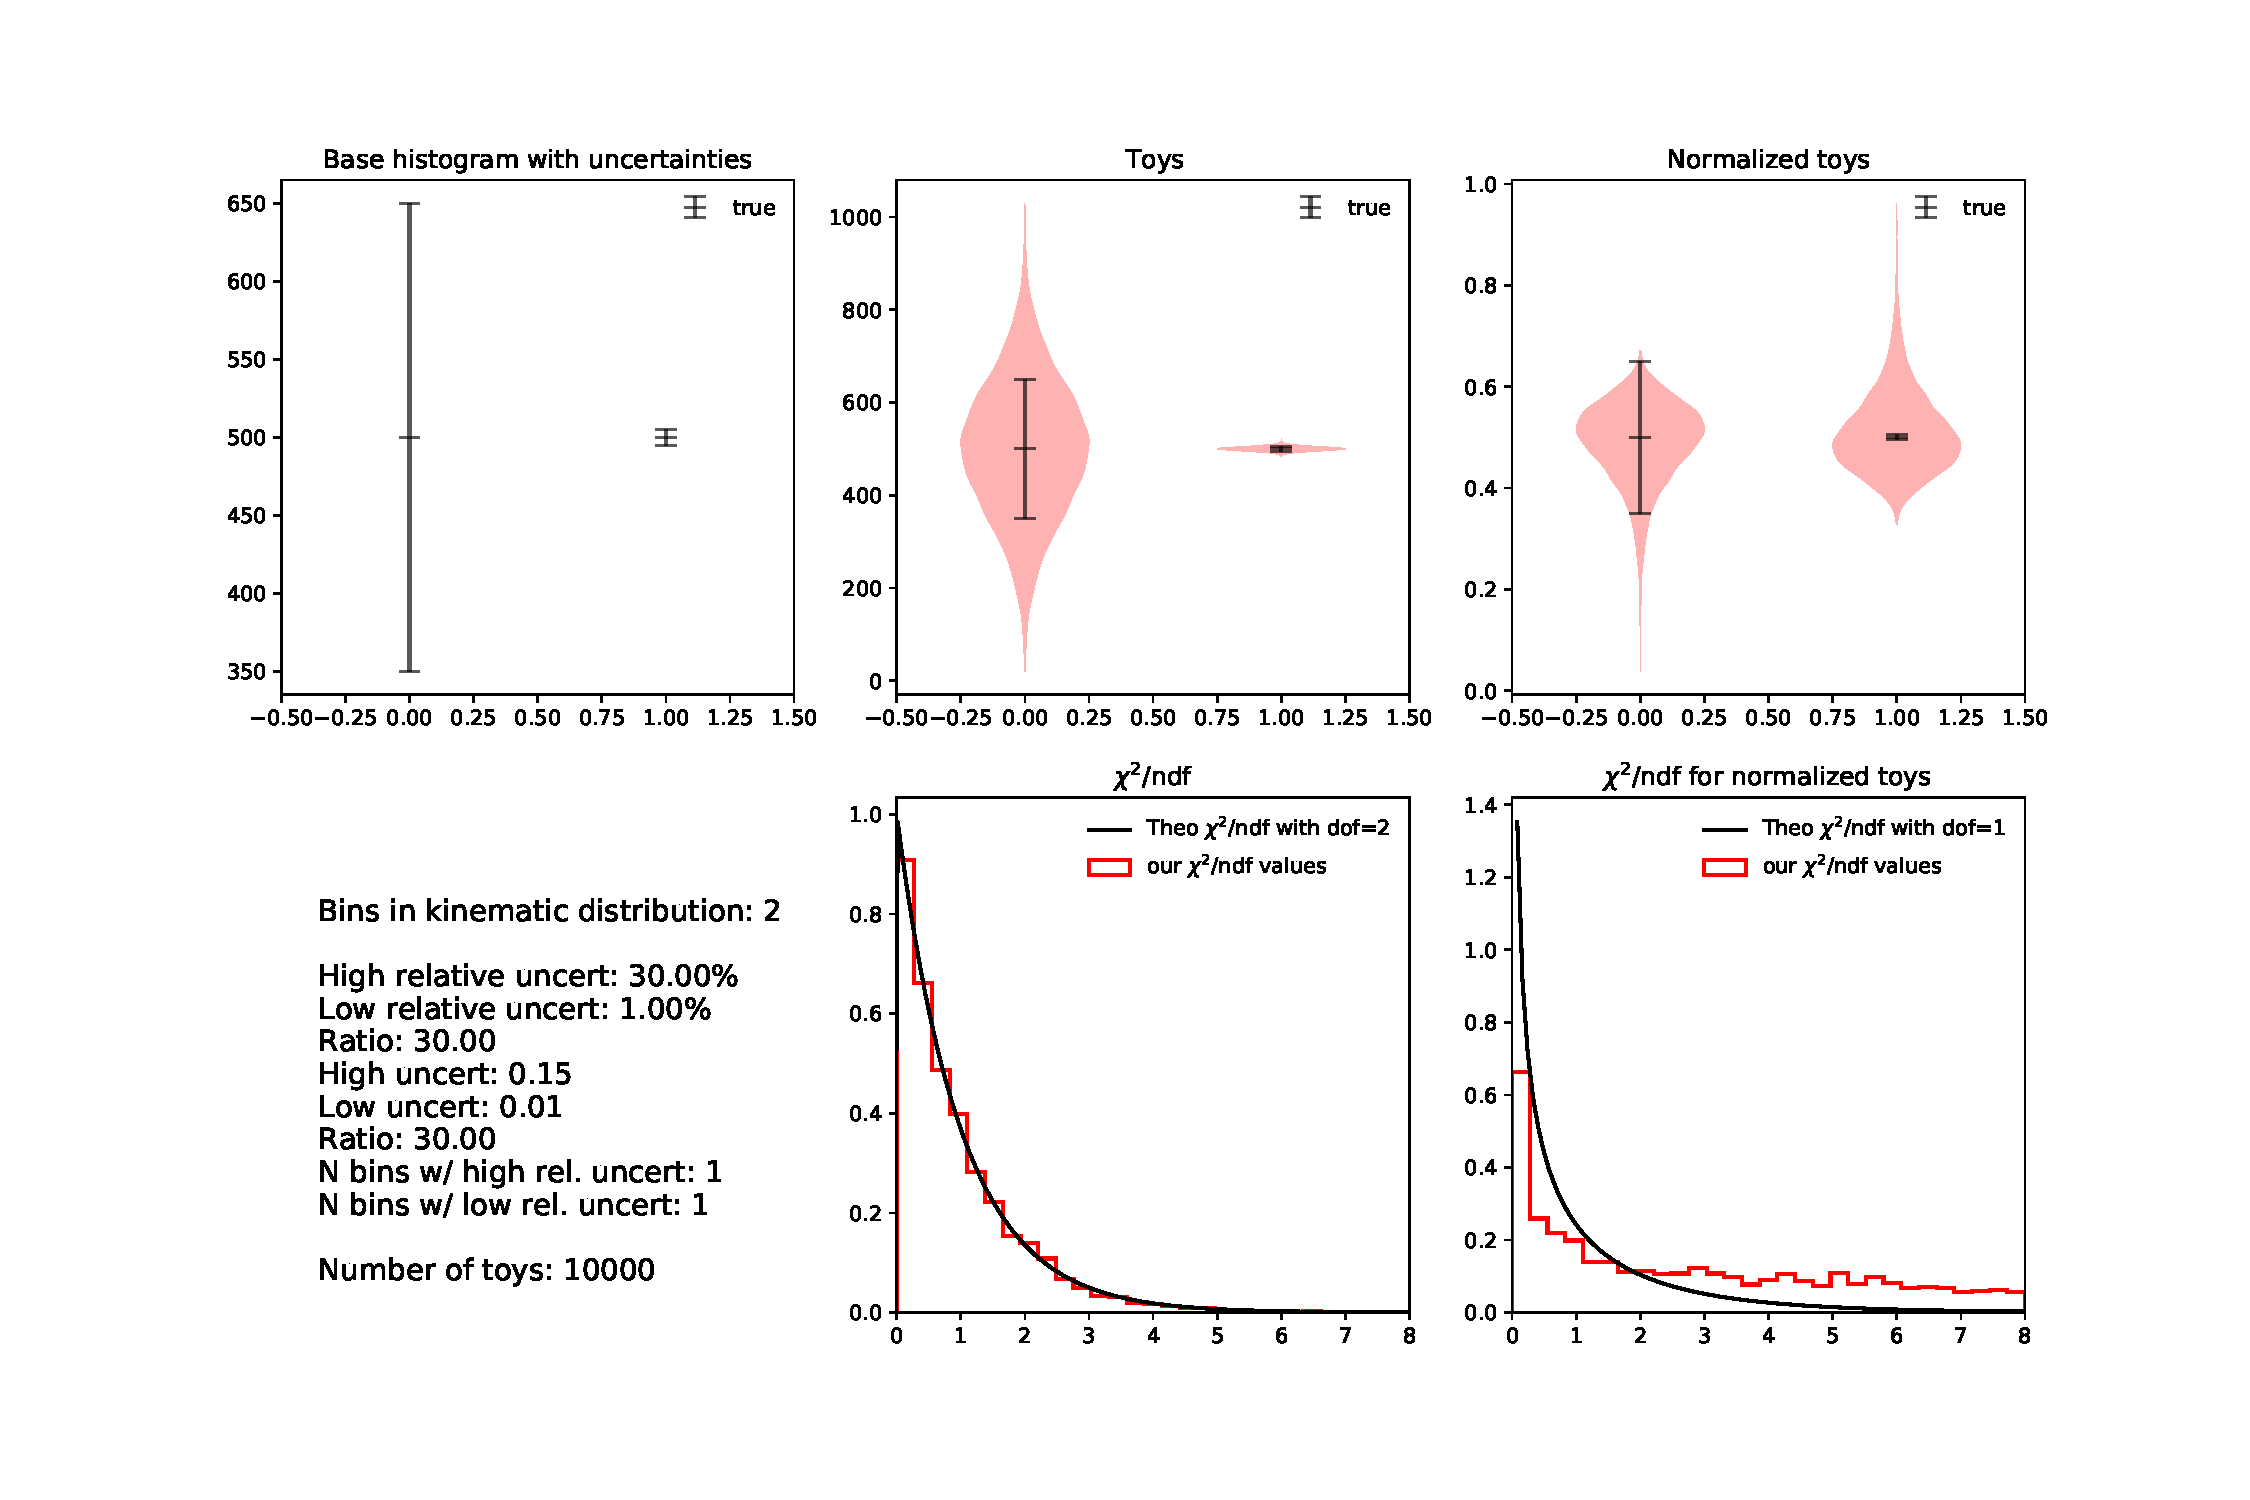
\includegraphics[width=12.3cm, trim=1cm 0cm 1cm 2.3cm, clip]{figures/chi2-normalization-puzzle-plots/2bins_30ratio.pdf}}
	\only<2>{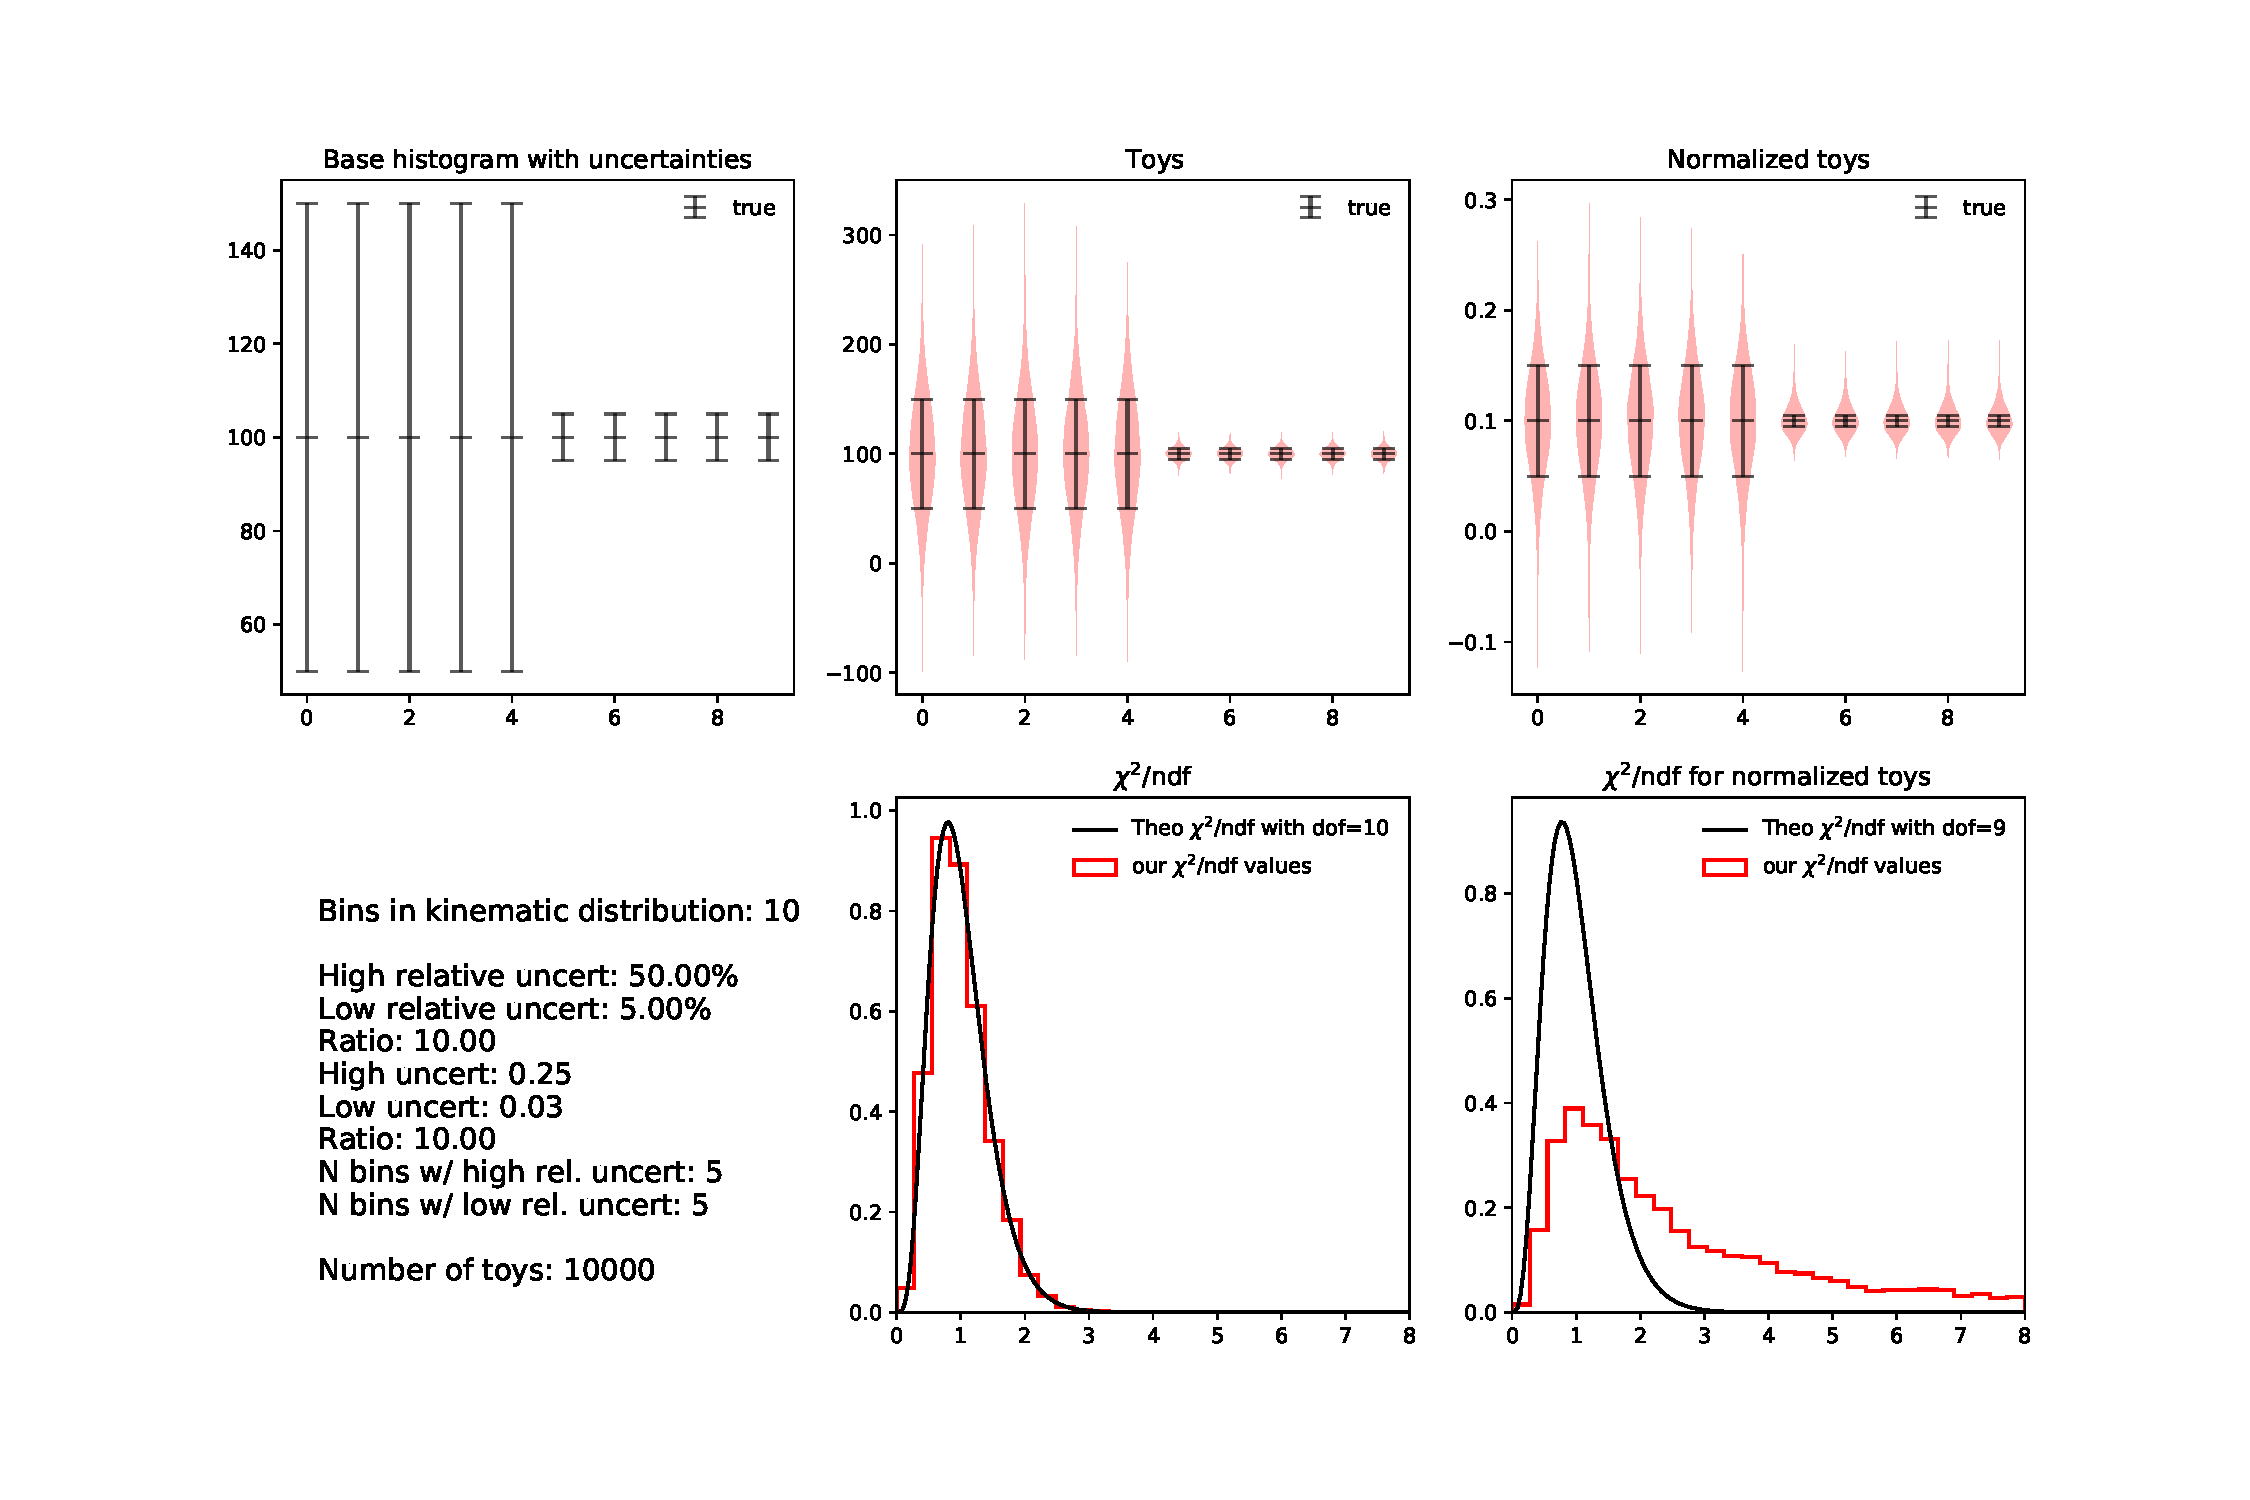
\includegraphics[width=12.3cm, trim=1cm 0cm 1cm 2.3cm, clip]{figures/chi2-normalization-puzzle-plots/10bins_10ratio.pdf}}
	\end{changemargin}
\end{frame}

\begin{frame}{The metric}{Validation}
	\begin{itemize}
		\item Let's test implementation \& approximation
		\item Generate toys according to sample and calculate $\chi^2$ distance to base distribution \srem{(or other half of toys)}
	\end{itemize}
	\begin{figure}
		\centering
		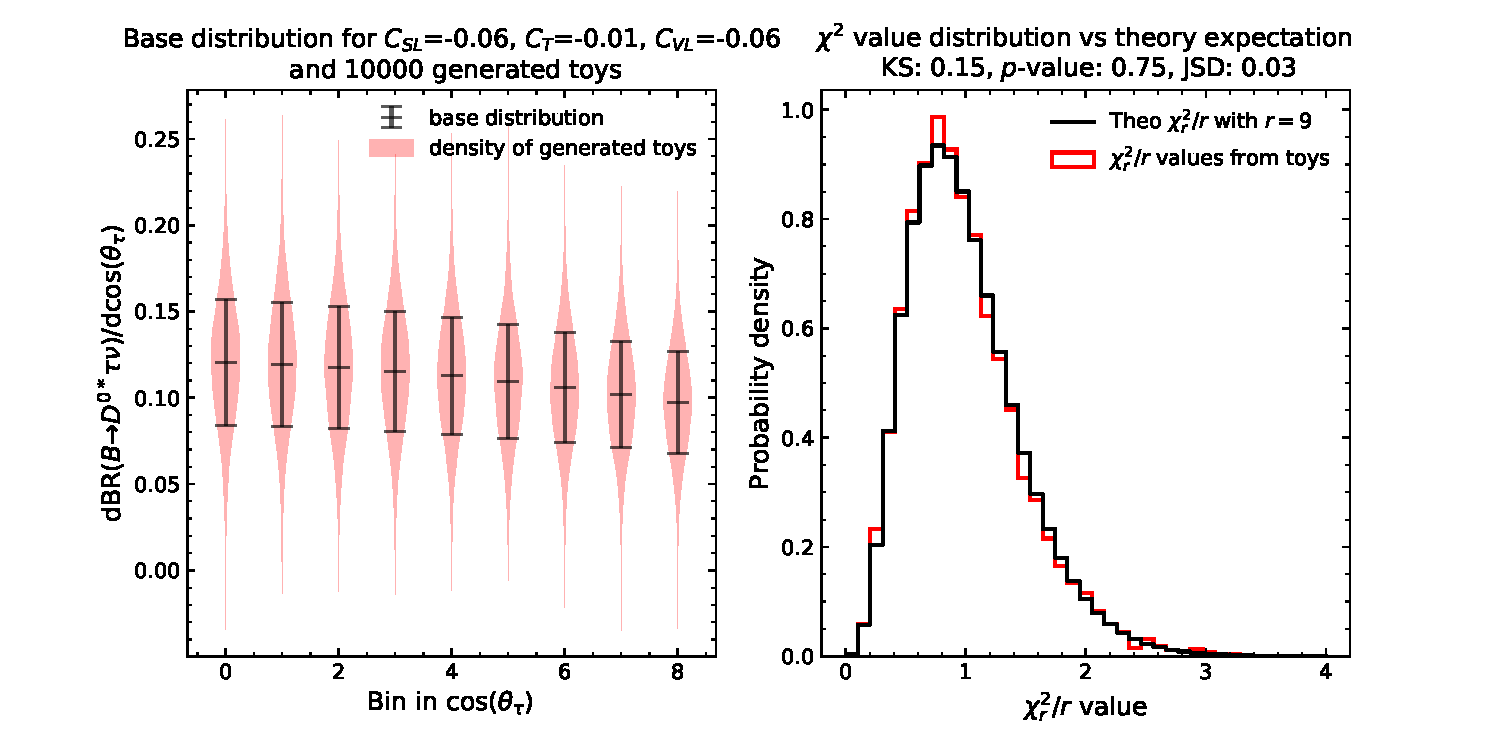
\includegraphics[width=12cm]{figures/erratum-plots/toy_experiment_demo.pdf}
	\end{figure}
\end{frame}

\begin{frame}{The metric}{Expanding to a metric between clusters}
	\begin{itemize}
		\item So far we have a metric between histograms $H_{1,2}$ corresponding to parameter points $p_{1,2}$
		\item Pull back to metric between points in parameter space: \hhl{$d(p_1,p_2):=\chi^2(H_1, H_2)/(N-1)$} \srem{divided out degrees of freedom such that expectation value is 1 under null hypothesis}
		\item Our clustering algorithm will be iterative: 
		\begin{enumerate}
			\item start with some clusters
			\item merge clusters that look similar
			\item repeat until stopping criterion is reached
		\end{enumerate}
		$\Lra$ Actually need a \hhl{metric between clusters}!
	\end{itemize}
\end{frame}

\begin{frame}[t]{Example: Hierarchical Clustering}
	\vspace{0.5cm}
   \centering
	\only<+>{
		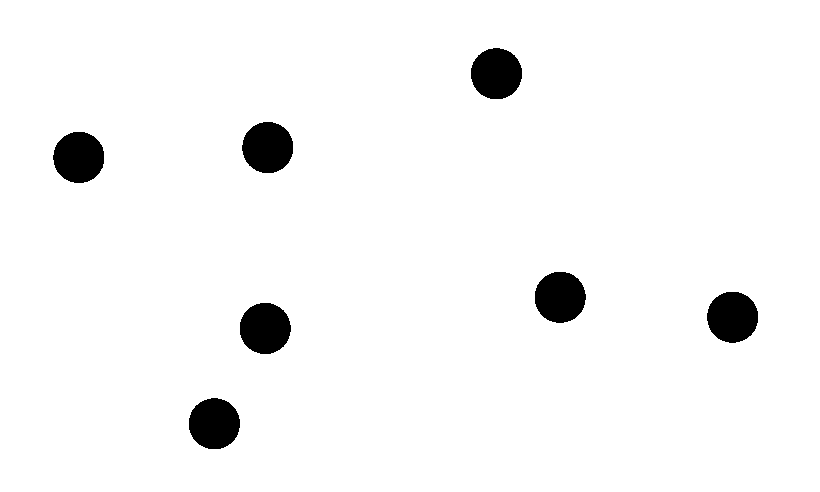
\includegraphics[width=10cm]{figures/hierarchy/step0.pdf}\\[2ex]
		Step 0: 7 points in the parameter space
	}
	\only<+>{
		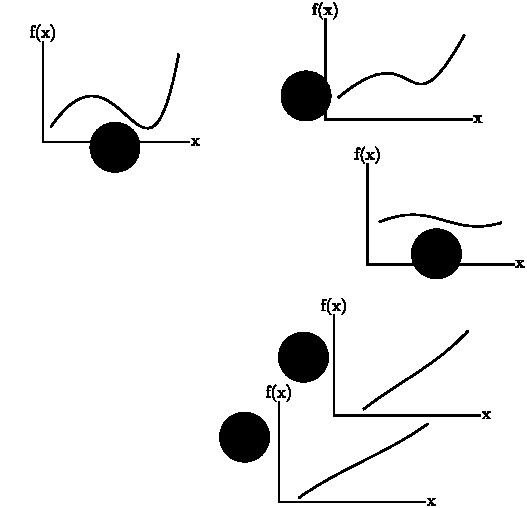
\includegraphics[width=10cm]{figures/hierarchy/step0_curves.pdf}\\[2ex]
		Step 0: 7 points in the parameter space = 7 distributions
	}
	\only<+>{
		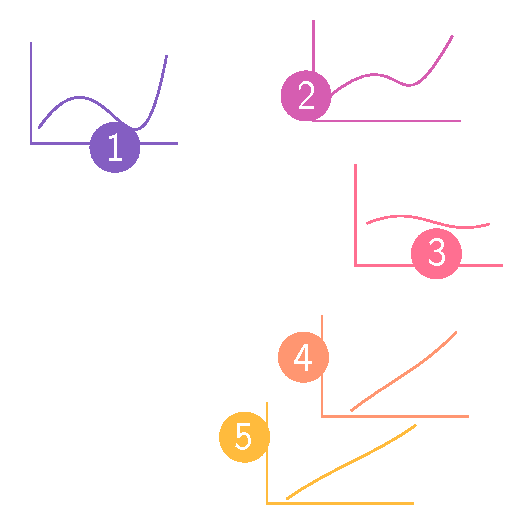
\includegraphics[width=10cm]{figures/hierarchy/step1_curves.pdf}\\[2ex]
		Step 1: Every point is its own cluster
	}
	\only<+>{
		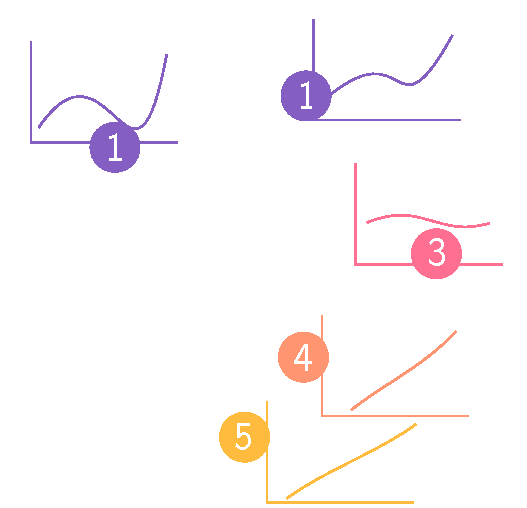
\includegraphics[width=10cm]{figures/hierarchy/step2_curves.pdf}\\[2ex]
		Step 1: Distributions from cluster 6 and 7 were the most similar $\Lra$ Merged!
	}
	\only<+>{
		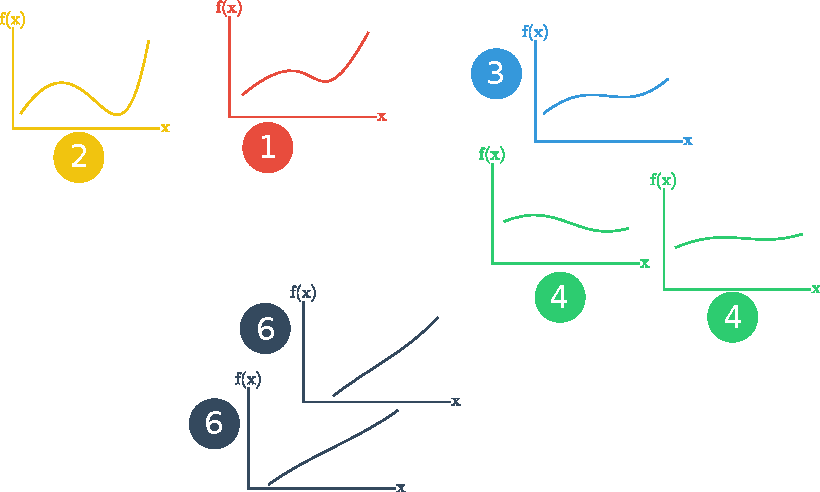
\includegraphics[width=10cm]{figures/hierarchy/step3_curves.pdf}\\[2ex]
		Step 1: Cluster 4 and 5 were the next most similar clusters $\Lra$ Merged!
	}
	\only<+>{
		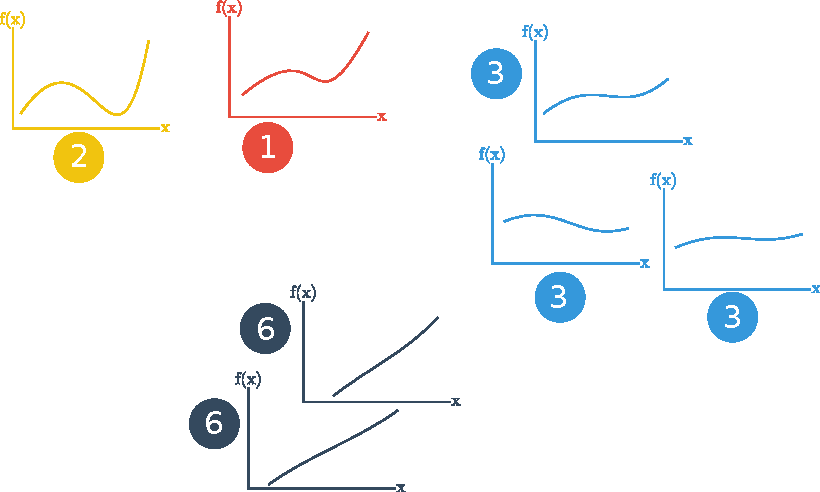
\includegraphics[width=10cm]{figures/hierarchy/step4_curves.pdf}\\[2ex]
		Step 1: 4 clusters remaining
	}
	\only<+>{
		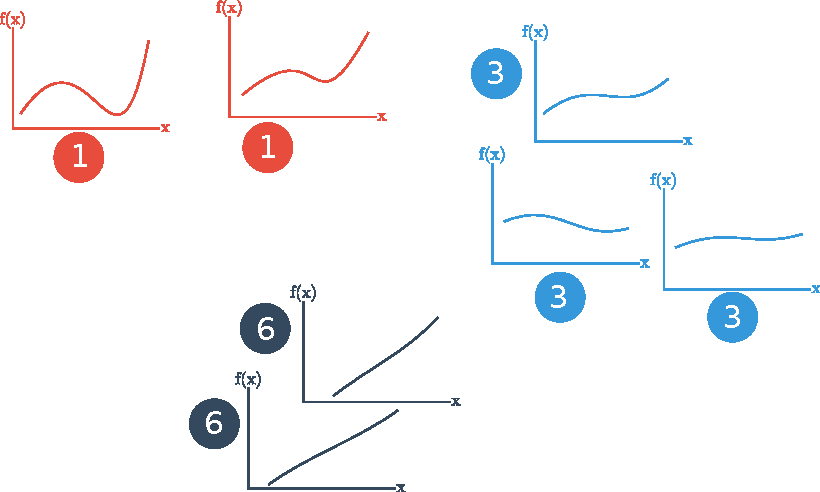
\includegraphics[width=10cm]{figures/hierarchy/step5_curves.pdf}\\[2ex]
		Step 1: 3 clusters remaining
	}
	\only<+>{
		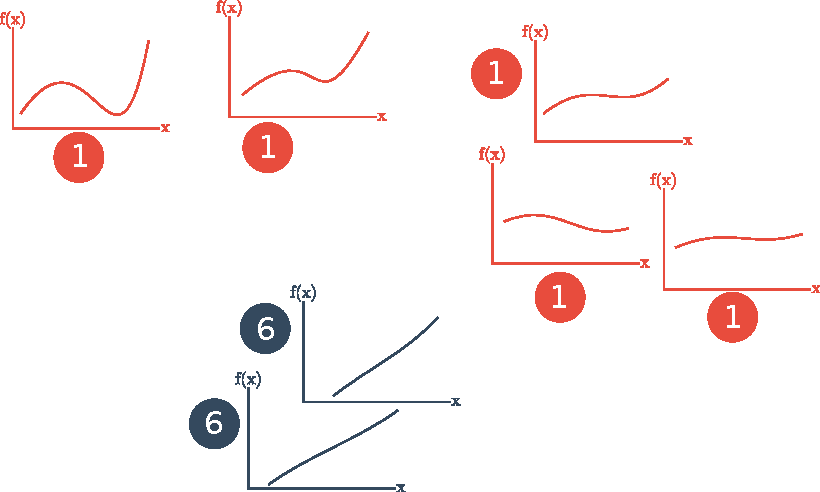
\includegraphics[width=10cm]{figures/hierarchy/step6_curves.pdf}\\[2ex]
		Step 1: 2 clusters remaining
	}
	\only<+>{
		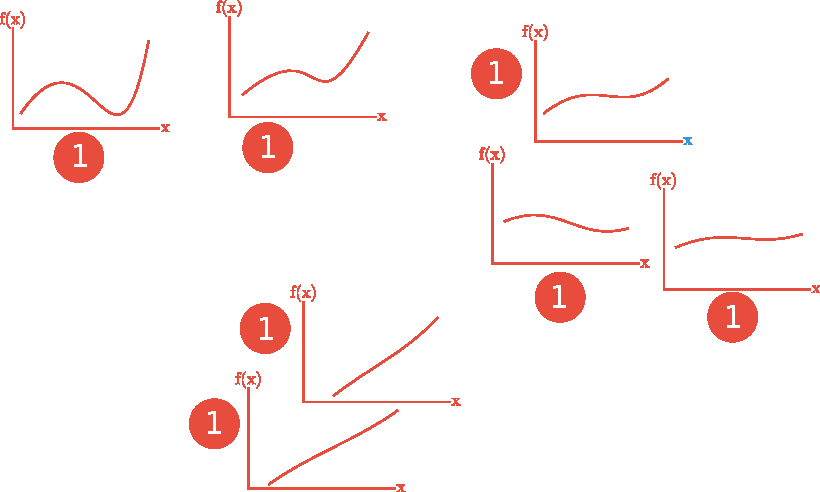
\includegraphics[width=10cm]{figures/hierarchy/step7_curves.pdf}\\[2ex]
		Step 1: 1 cluster remaining
	}
	
%	}
\end{frame}